\section{Thảo luận}
\label{sec:discussion}

Mục này giải thích các kết quả ở Mục~\ref{sec:results}: sai số của mô hình RUL,
thời điểm cảnh báo, sự khác biệt giữa hai biểu diễn HGB126/HGB169 và khả năng
chuyển miền sang các subset khác. Các số liệu chẩn đoán dùng
trong mục này được tính lại từ artifact đã có bằng
\filepath{scripts/report_error_diagnostics.py}, không huấn luyện lại mô hình.

\subsection{Sai số của mô hình RUL đến từ đâu}
\label{sec:disc-error}
Bảng~\ref{tab:oof-by-rul} và Hình~\ref{fig:oof-pred-true} chia sai số OOF của
HGB126 trên train theo RUL thật. Mô
hình dự đoán tốt ở cuối vòng đời: MAE chỉ 3,67 cycles khi RUL thật không quá 30.
Sai số tăng dần khi RUL lớn hơn, và thay đổi hẳn tính chất khi RUL vượt khoảng
150 cycles. Ở vùng này, dự đoán trung bình gần như không đổi, quanh 145--147
cycles, bất kể RUL thật là 160 hay 300. Nói cách khác, mô hình đã tự học ra một
``trần'' khoảng 145 cycles, và mọi động cơ còn xa thời điểm hỏng đều bị dự đoán
gần mức đó.

\begin{table}[H]
\centering
\caption[Sai số OOF theo RUL]{Sai số OOF của HGB trên 17.731 window train, chia theo RUL thật.
Sai số có dấu bằng dự đoán trừ thật.}
\label{tab:oof-by-rul}
\small
\begin{tabular}{lrrrr}
\toprule
RUL thật (cycles) & Số window & MAE & Sai số có dấu trung bình & Dự đoán trung bình\\\midrule
0--30 & 3.100 & 3,67 & $+1{,}47$ & 16,47\\
31--60 & 3.000 & 10,68 & $+5{,}59$ & 51,09\\
61--90 & 3.000 & 20,85 & $+14{,}52$ & 90,02\\
91--125 & 3.392 & 22,81 & $+12{,}88$ & 120,61\\
126--150 & 1.999 & 20,82 & $-2{,}87$ & 134,73\\
151--200 & 2.226 & 30,25 & $-23{,}30$ & 147,16\\
201--361 & 1.014 & 91,29 & $-91{,}29$ & 145,36\\
\bottomrule
\end{tabular}
\end{table}

\begin{figure}[H]
\centering
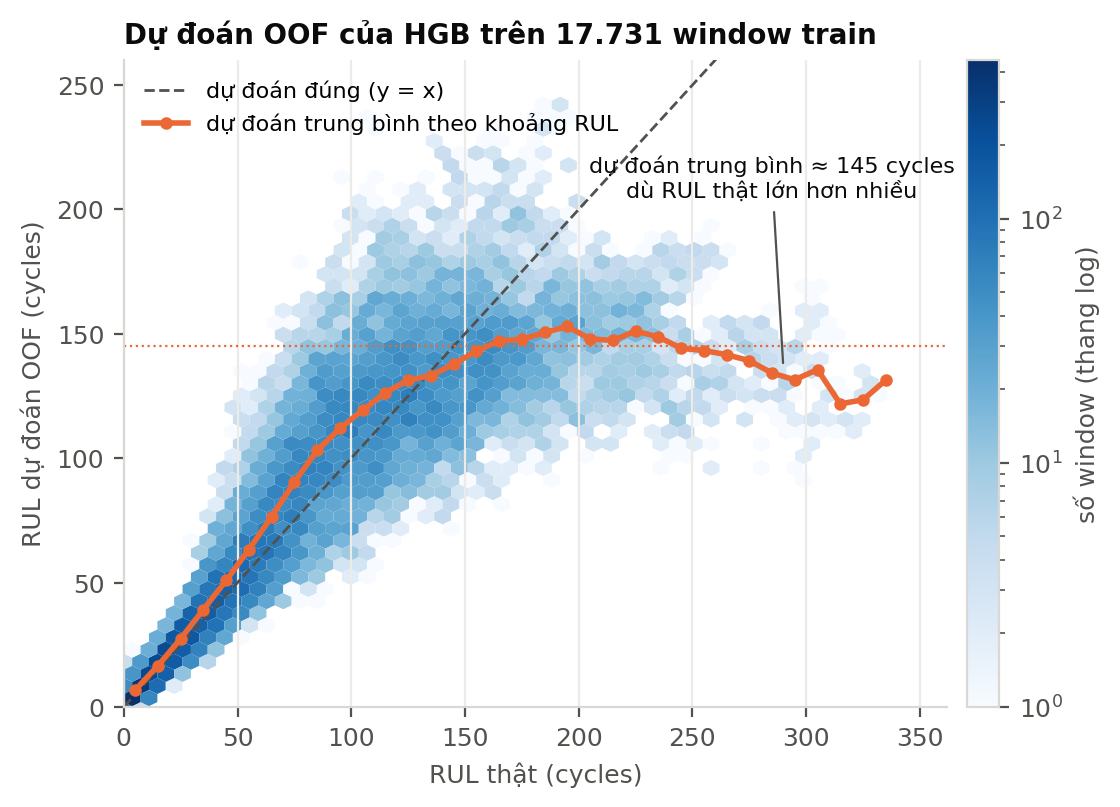
\includegraphics[width=0.6\linewidth]{../outputs/diagnostics/figures/oof_pred_vs_true.png}
\caption[RUL OOF so với thật]{RUL dự đoán OOF so với RUL thật. Đường cam là dự đoán trung bình theo
từng khoảng 10 cycles: bám sát đường chéo khi RUL nhỏ, nhưng dừng quanh 145 cycles
khi RUL thật lớn hơn khoảng 150.}
\label{fig:oof-pred-true}
\end{figure}

Hiện tượng này phù hợp với hình dạng của tín hiệu. Hình~\ref{fig:hi-trajectories}
cho thấy Health Index của các động cơ gần như đi ngang, chỉ dao động quanh một
mức, trong phần lớn vòng đời và chỉ giảm rõ ở giai đoạn cuối. Khi động cơ còn
khỏe, sensor chủ yếu phản ánh dao động đo và khác biệt ban đầu giữa các động cơ,
nên khó phân biệt một động cơ còn 160 cycles với một động cơ còn 300 cycles.
Kết quả này phù hợp với giả thuyết rằng biểu diễn hiện tại chứa ít tín hiệu phân
biệt RUL xa; dữ liệu hiện có chưa đủ để khẳng định một giới hạn thông tin cố định.
Nó cũng giải thích vì sao MAE cross-validation (20,21
cycles) cao hơn MAE test (15,35 cycles): 29,5\% số window train có RUL thật trên
125, trong khi RUL thật của test chỉ từ 7 đến 145.

\begin{figure}[H]
\centering
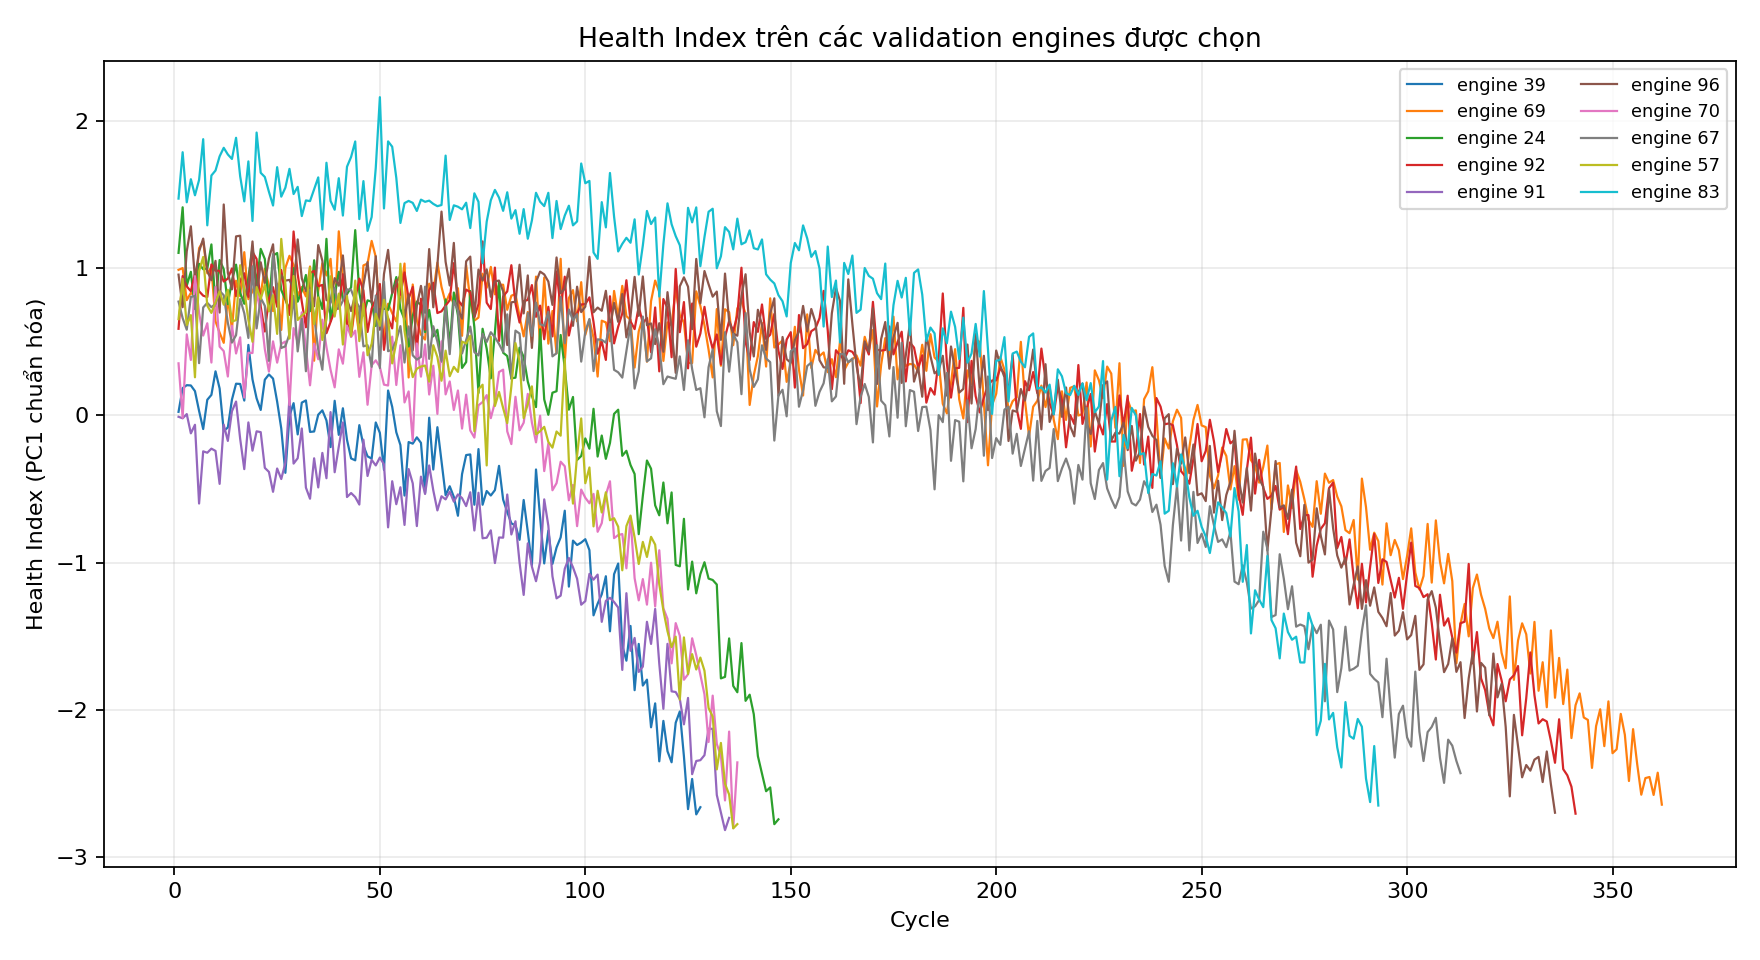
\includegraphics[width=0.6\linewidth]{../outputs/timeseries/figures/health_index_selected_engines.png}
\caption[Health Index của 10 động cơ]{Health Index theo cycle của 10 động cơ train được chọn ở Mục~\ref{sec:arima-method}.
Chỉ số gần như đi ngang ở phần lớn vòng đời và giảm rõ ở giai đoạn cuối.}
\label{fig:hi-trajectories}
\end{figure}

Ở vùng giữa (RUL 61--125), mô hình có xu hướng dự đoán cao hơn thật khoảng
13--15 cycles. Mười sai số lớn nhất trên test rơi vào các động cơ có RUL thật
77--137, phần lớn trùng với vùng này, và đều là dự đoán cao; riêng mười trường hợp
này chiếm 75,5\% NASA score. Như vậy, sai số test không phải ngẫu nhiên mà lặp lại
đúng xu hướng đã thấy trên OOF.

So với nghiên cứu liên quan, Li và cộng sự báo cáo RMSE 12,61 cycles trên FD001
với CNN khi cắt nhãn ở 125 cycles, và 13,32 cycles khi không cắt
nhãn~\cite{li2018rul}. RMSE của báo cáo là 20,54 cycles. Hai kết quả không so sánh
trực tiếp được, vì Li và cộng sự dùng 14 sensor, cách chuẩn hóa và mô hình khác.
Tuy vậy, khoảng cách khoảng 7 cycles so với cả phương án không cắt nhãn cho thấy
việc chỉ cắt nhãn có thể chưa đủ: sáu thống kê trên window 30 cycles có thể đã
làm mất một phần thông tin về hình dạng chuỗi mà CNN khai thác được.

\subsection{Vì sao gần một nửa cảnh báo bị trễ}
\label{sec:disc-warning}
Cảnh báo trễ không phân bố đều giữa các động cơ. 49 động cơ bị cảnh báo sau
ngưỡng có tuổi thọ trung bình 182,8 cycles, trong khi 44 động cơ được cảnh báo
trước ngưỡng có tuổi thọ trung bình 229,1 cycles. Hệ số tương quan giữa tuổi thọ
và độ lệch cảnh báo $\delta_i$ là $-0{,}56$: động cơ càng ngắn đời thì càng bị
cảnh báo muộn (Hình~\ref{fig:warning-lifetime}).

\begin{figure}[H]
\centering
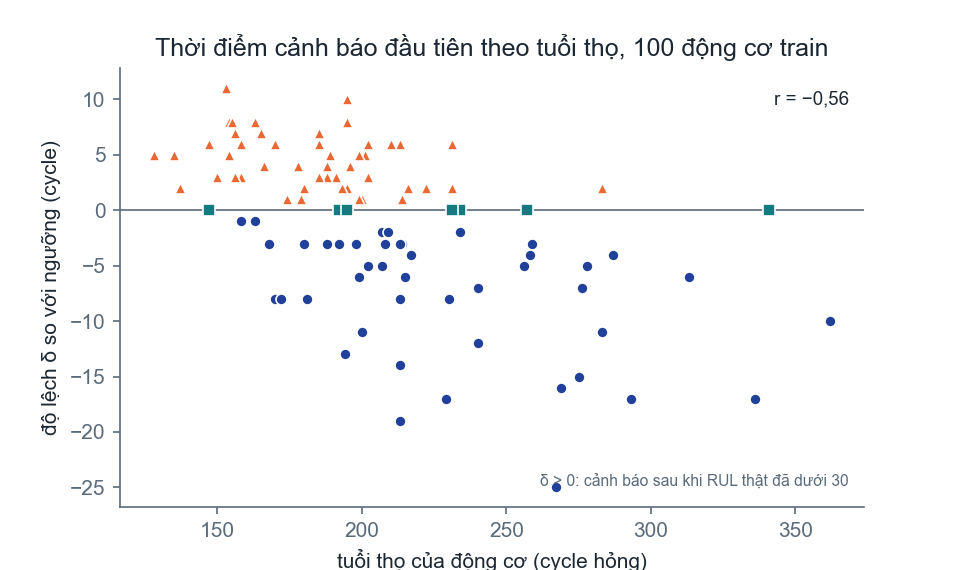
\includegraphics[width=0.62\linewidth]{../outputs/diagnostics/figures/warning_vs_lifetime.png}
\caption[Cảnh báo theo tuổi thọ]{Độ lệch của cảnh báo đầu tiên so với ngưỡng theo tuổi thọ của 100 động
cơ train. Cảnh báo trễ (tam giác cam) tập trung ở các động cơ hỏng trước khoảng
cycle 230.}
\label{fig:warning-lifetime}
\end{figure}

Một cách giải thích là mô hình học một quan hệ ``trung bình'' giữa mức sensor và
RUL. Động cơ ngắn đời suy giảm nhanh hơn trung bình, nên tại cùng một mức sensor,
RUL thật của chúng thấp hơn điều mô hình kỳ vọng. Kết quả là RUL dự đoán giảm
xuống dưới 30 muộn hơn thực tế. Điều này nhất quán với sai số dương ở vùng RUL
31--90 trong Bảng~\ref{tab:oof-by-rul}. Đặc trưng độ dốc trong window 30 cycles
lẽ ra phải phản ánh tốc độ suy giảm, nhưng trên 30 cycles, xu hướng thật có thể
bị dao động ngắn hạn che khuất. Phân tích trailing mean chỉ cho thấy biến động
được làm dịu trong mô tả tín hiệu; nó không chứng minh dữ liệu có nhiễu đo đã
biết hoặc rằng smoothing chắc chắn cải thiện RUL.

Từ góc độ ứng dụng, đây là loại lỗi nguy hiểm hơn cả: động cơ hỏng nhanh nhất lại
là động cơ nhận cảnh báo muộn nhất. Một ngưỡng cố định 30 cycles vì vậy chưa đủ.
Muốn bảo đảm lead time tối thiểu, ngưỡng cần có biên an toàn, hoặc mô hình cần
biết được tốc độ suy giảm riêng của từng động cơ. Cũng cần nhớ rằng các con số
cảnh báo được tính trên cùng tập OOF đã dùng để chọn mô hình, nên trên dữ liệu
mới, tỷ lệ cảnh báo trễ có thể còn cao hơn.

\subsection{Vì sao mô hình FD001 không chuyển được sang subset khác}
\label{sec:disc-transfer}
Bảng~\ref{tab:transfer-diagnostics} và Hình~\ref{fig:transfer-shift} cho thấy mô
hình FD001 thất bại theo hai kiểu khác nhau.

\begin{figure}[H]
\centering
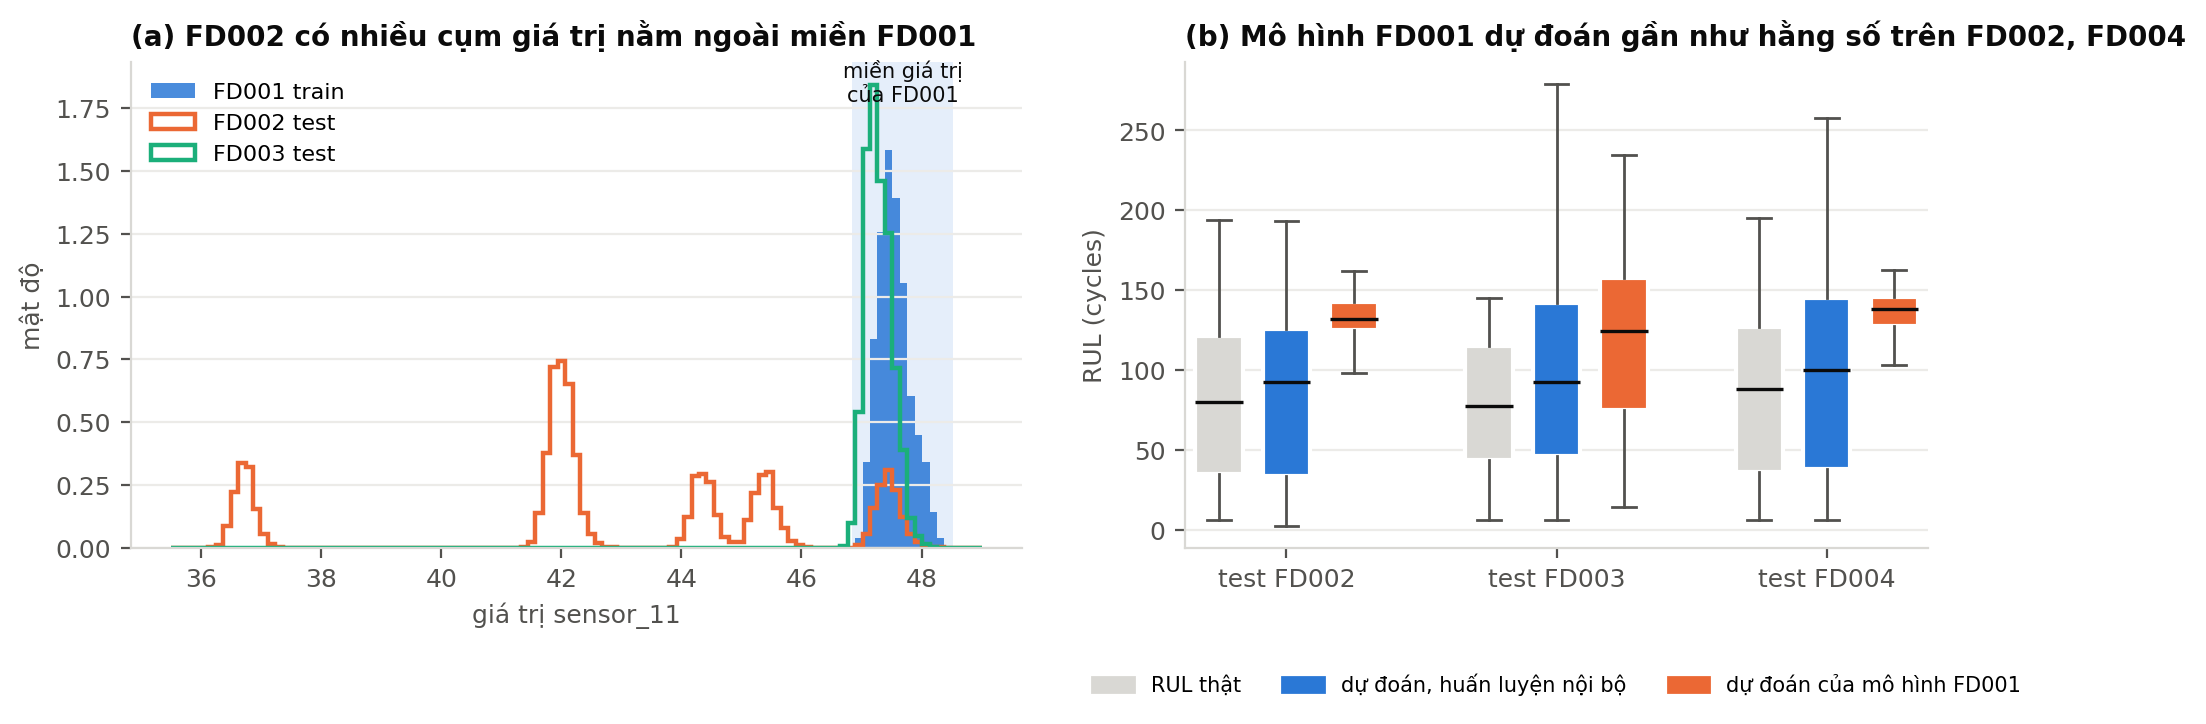
\includegraphics[width=\linewidth]{../outputs/diagnostics/figures/transfer_shift.png}
\caption[Dịch chuyển phân phối sensor]{(a) Phân phối \texttt{sensor\_11}: FD003 nằm trong miền giá trị của FD001,
còn FD002 tách thành nhiều cụm theo điều kiện vận hành, phần lớn nằm ngoài miền
này (FD004 có dạng tương tự FD002). (b) Phân phối RUL thật và RUL dự đoán trên test
của từng subset: mô hình FD001 cho dự đoán rất hẹp trên FD002 và FD004.}
\label{fig:transfer-shift}
\end{figure}

\begin{table}[H]
\centering
\caption[Chẩn đoán chuyển miền]{Chẩn đoán dự đoán chuyển miền (window 10). ``Trong miền FD001'' là tỷ lệ
trung bình giá trị test của 9 sensor có xu hướng nằm trong khoảng min--max của
train FD001. TB: trung bình.}
\label{tab:transfer-diagnostics}
\small
\begin{tabular}{l>{\raggedleft\arraybackslash}p{1.7cm}>{\raggedleft\arraybackslash}p{1.7cm}>{\raggedleft\arraybackslash}p{1.6cm}>{\raggedleft\arraybackslash}p{1.9cm}>{\raggedleft\arraybackslash}p{1.6cm}}
\toprule
Đánh giá & Trong miền FD001 & Sai số có dấu TB & Tỷ lệ dự đoán cao & Độ lệch chuẩn dự đoán & RUL thật TB\\\midrule
FD001 $\rightarrow$ FD002 & 15,2\% & $+50{,}79$ & 81\% & 13,33 & 81,19\\
FD001 $\rightarrow$ FD003 & 94,7\% & $+45{,}34$ & 83\% & 55,01 & 75,32\\
FD001 $\rightarrow$ FD004 & 14,1\% & $+49{,}39$ & 79\% & 12,72 & 86,55\\
FD002 $\rightarrow$ FD002 & -- & $+2{,}64$ & 54\% & 52,53 & 81,19\\
FD003 $\rightarrow$ FD003 & -- & $+22{,}85$ & 75\% & 63,11 & 75,32\\
FD004 $\rightarrow$ FD004 & -- & $+12{,}18$ & 62\% & 62,59 & 86,55\\
\bottomrule
\end{tabular}
\end{table}

Với FD002 và FD004, chỉ khoảng 14--15\% giá trị sensor của test nằm trong miền giá
trị mà mô hình đã thấy khi huấn luyện, do sáu điều kiện vận hành đẩy mức sensor
ra xa điều kiện duy nhất của FD001. Mô hình cây không ngoại suy được: mọi giá trị
nằm ngoài miền huấn luyện đều rơi vào các lá ở biên. Hệ quả là dự đoán gần như
hằng số (độ lệch chuẩn khoảng 13 cycles, so với khoảng 52--63 khi huấn luyện nội
bộ) và cao hơn RUL thật khoảng 50 cycles. Như vậy, thất bại ở đây nhiều khả năng
đến từ dịch chuyển phân bố đầu vào (covariate shift) do điều kiện vận hành, hơn là
từ việc mô hình hiểu sai quá trình suy giảm. Khi tự huấn luyện trên FD002, mô hình gần
như không lệch (sai số có dấu $+2{,}64$), cho thấy thông tin để dự đoán vẫn có sẵn
trong dữ liệu.

FD003 là trường hợp khác. Giá trị sensor gần như nằm hoàn toàn trong miền FD001
(94,7\%) và dự đoán vẫn biến thiên (độ lệch chuẩn 55), tức mô hình có ``phản
ứng'' với dữ liệu. Tuy nhiên, dự đoán vẫn cao hơn thật trung bình 45 cycles. FD003
có thêm dạng lỗi fan; một giả thuyết hợp lý là dạng lỗi này làm sensor thay đổi
theo kiểu khác với suy giảm HPC mà mô hình đã học, nên động cơ trông ``khỏe'' hơn
thực tế. Ngay cả khi huấn luyện nội bộ, FD003 vẫn bị dự đoán cao trung bình 22,85
cycles, cho thấy hai dạng lỗi trong cùng một tập là khó hơn cho cách biểu diễn
hiện tại.

Hai kiểu thất bại này cần hai cách xử lý khác nhau: FD002 và FD004 cần loại bỏ
ảnh hưởng của điều kiện vận hành trước khi tạo đặc trưng; FD003 cần dữ liệu huấn
luyện có dạng lỗi tương ứng hoặc đặc trưng phân biệt được dạng lỗi.

\subsection{Vì sao thử nghiệm cải thiện không thành công}
Các hướng đã thử trong nested CV (đổi window, chỉnh siêu tham số và tăng trọng
số vùng RUL thấp) chưa tìm được cấu hình mới vượt bộ tiêu chí đã chốt. Đợt HGB
bổ sung cho thấy thêm window 10 có thể giảm RMSE trajectory nhưng làm xấu
endpoint hoặc on-time; profile 30 cycles đầu còn làm RMSE tăng. Pilot
similarity-based RUL cũng không đạt: RMSE 36,543--37,173 so với 28,835 của HGB
169 trên cùng panel 3 fold, và bị dừng trước full study. Các kết quả này không
chứng minh rằng mọi kiến trúc mới đều kém; chúng chỉ cho thấy các thay đổi đã
được kiểm tra chưa giải quyết được hai nguyên nhân sai số chính: tín hiệu đầu
vòng đời khó phân biệt RUL xa và tốc độ suy giảm khác nhau giữa các động cơ.

Alignment audit cho thấy HGB169 tốt hơn HGB126 trên panel trajectory và endpoint
chung, nên HGB169 được chọn làm predictor candidate chính trong phạm vi bằng
chứng hiện có. Kết luận này có điều kiện: so sánh dựa trên dự đoán đã lưu,
bootstrap không bao gồm bất định fit lại, và run lịch sử đã được kiểm tra trước;
chưa có một lần refit mù độc lập để xác nhận. Vì vậy metric test của HGB126 vẫn
được giữ như baseline lịch sử; báo cáo không dùng metric test của HGB169 để chọn
predictor.

\subsection{Ý nghĩa đối với xử lý dữ liệu lớn}
Với 265.256 quan sát trên cả bốn subset, dữ liệu C-MAPSS vẫn vừa trong bộ nhớ
của một máy, nên Pandas đủ dùng. Giá trị của phần dữ liệu lớn trong báo cáo nằm ở
cách tổ chức: kiểm tra contract trước khi xử lý, lưu dữ liệu theo lớp, và có một
implementation ETL bằng PySpark cho kết quả giống hệt Pandas. Nhờ đó, khi dữ liệu
tăng lên (nhiều đội động cơ, tần suất lấy mẫu cao hơn), phần ETL có thể chuyển
sang Spark với bằng chứng parity sẵn có. Đợt bổ sung đã triển khai sáu thống kê
cho 21 sensor bằng Spark và kiểm tra toàn bộ rolling features ở scale 1$\times$.
Benchmark local có I/O được trình bày ở Bảng~\ref{tab:followup-benchmark}.

Để tránh đồng nhất Big Data với riêng kích thước tập tin, Bảng~\ref{tab:big-data-5v}
đối chiếu năm khía cạnh của bài toán với bằng chứng thực tế và giới hạn tương ứng.
Đây là pipeline batch theo hướng Big Data; báo cáo không gán cho C-MAPSS hiện tại
quy mô phân tán mà dữ liệu chưa có.

\begin{table}[H]
\centering
\caption[Phạm vi Big Data theo 5V]{Đối chiếu 5V, bằng chứng và giới hạn của pipeline.}
\label{tab:big-data-5v}
\small
\begin{tabularx}{\linewidth}{L{2.0cm}L{6.0cm}X}
\toprule
Khía cạnh & Bằng chứng trong báo cáo & Giới hạn hiện tại \\\midrule
Volume & 265.256 quan sát từ bốn subset; dữ liệu raw khoảng 46 MB; kích thước bảng được ghi ở từng bước ETL. & Vẫn vừa bộ nhớ một máy; benchmark nhân bản chỉ đo chi phí kỹ thuật. \\
Velocity & Pipeline xử lý batch theo từng subset, có thể chạy lại từ file raw và Parquet. & Chưa có streaming, ingest liên tục hoặc yêu cầu độ trễ thời gian thực. \\
Variety & Có 21 sensor, 3 operational settings, khóa engine/cycle, chuỗi run-to-failure và nhãn RUL; bốn subset thể hiện các tổ hợp điều kiện vận hành và dạng lỗi khác nhau, được lưu qua text, Parquet, SQLite và bảng đặc trưng. & Các định dạng lưu trữ vẫn xuất phát từ cùng nguồn cảm biến dạng bảng; chưa có nhiều nguồn dị thể hoặc dữ liệu phi cấu trúc. \\
Veracity & Contract schema, kiểm tra khóa và cycle, kiểm tra giá trị thiếu, hash và parity Pandas--PySpark. & Chưa kiểm chứng với lỗi cảm biến và dữ liệu thiếu của hệ thống thực. \\
Value & RUL, cảnh báo sớm và đánh giá chuyển miền cho FD001--FD004. & Chưa có chi phí bảo trì, downtime hoặc KPI kinh tế. \\
\bottomrule
\end{tabularx}
\end{table}

\subsection{Giới hạn}
\label{sec:limitations}
\paragraph{Về dữ liệu.} C-MAPSS là dữ liệu mô phỏng; động cơ thực tế có lỗi cảm
biến, dữ liệu thiếu và điều kiện vận hành phức tạp hơn. Dữ liệu cũng không có
chi phí bảo trì hay cách quy đổi cycle sang thời gian thực, nên báo cáo không thể
đánh giá giá trị kinh tế của cảnh báo.

\paragraph{Về đánh giá.} Metric test chỉ đo tại một điểm cắt mỗi động cơ, trong
khi trong vận hành, mô hình sẽ được gọi ở mọi cycle. Kết quả cảnh báo dùng lại
tập OOF đã dùng để chọn mô hình. Nhãn test FD001 đã được xem trước thử nghiệm
nested CV, nên test không còn hoàn toàn độc lập với thử nghiệm đó. So sánh giữa
window 10 và window 30 ở Mục~\ref{sec:res-transfer} không phải một thí nghiệm có
kiểm soát. Các giải thích trong Mục~\ref{sec:disc-error}--\ref{sec:disc-transfer}
là giả thuyết phù hợp với dữ liệu; thí nghiệm bổ sung dưới đây kiểm tra nhãn,
lịch sử và điều kiện vận hành nhưng chưa chứng minh cơ chế nhân quả.

\paragraph{Về hạ tầng.} Benchmark bổ sung đo Pandas và PySpark local, gồm đọc ghi
file. Spark ghi qua Arrow trên driver trong môi trường Windows; chưa đo distributed
writer hoặc cụm nhiều máy. Dữ liệu nhân bản
không làm tăng số mẫu khoa học độc lập.
Việc công bố nhiều file qua staging và rollback không phải atomic transaction
(giao dịch nguyên tử): chưa bảo đảm đọc/ghi đồng thời hoặc mất điện đột ngột. Đợt kiểm chứng mã
nguồn ngày 07/10/2026 chạy trên Windows; Linux mới được đối chiếu dependency
theo nền tảng và phiên bản từ lock, chưa chạy trực tiếp trong đợt này.

\subsection{Thí nghiệm bổ sung và hướng phát triển}
\label{sec:followup}
Ngày 29/09/2026, ba nghiên cứu nested GroupKFold 5$\times$3 được chạy theo
protocol ghi trước khi fit. FD001 dùng window 30, kết hợp cap
$R_{\max}\in\{110,125,140,\infty\}$ với bật/tắt 42 history features: độ lệch
so với mean 30 cycles đầu và slope trên toàn bộ prefix đã quan sát. Ví dụ,
feature ở cycle 40 không dùng cycle 41 trở đi. Chỉ cắt nhãn train, giữ nguyên
nhãn validation/test. HGB giữ cấu hình baseline và tổng trọng số mỗi engine bằng 1.

FD002/FD004 dùng window 10, so baseline với thêm settings và chuẩn hóa sensor
theo sáu cụm điều kiện vận hành. Scaler, KMeans và mean/std theo cụm đều chỉ fit
trên training engines của từng fold. Đây là đánh giá trong từng subset, không
phải chuyển trực tiếp từ FD001. FD001 yêu cầu CI 95\% của delta low-RUL MAE và
late rate đều dưới 0, overall MAE/burden không tăng; hai subset còn lại yêu cầu
upper CI delta overall MAE dưới 0. Bootstrap dùng 10.000 lần lấy lại engine,
có điều kiện theo dự đoán đã fit. Test lịch sử đã được xem, nên đây là follow-up
khám phá; test không quyết định lựa chọn. Chi tiết cấu hình, CI và từng metric
được lưu tại \filepath{experiments/FOLLOWUP_20260929.md}.

% Generated by scripts/build_followup_summary.py; author: Phan Nguyễn Mai Phương, MSHV 25002711.
\begin{table}[H]\centering\small
\caption[Nested CV bổ sung]{Follow-up nested CV: MAE vòng ngoài và test (cycles). Tiêu chí được chốt riêng cho từng nghiên cứu.}
\label{tab:followup}\begin{tabular}{lrrrr}\toprule
Subset & Outer baseline & Outer chọn & Test chọn & Đạt tiêu chí\\\midrule
FD001 & 20,21 & 20,30 & 13,05 & Không\\
FD002 & 29,29 & 28,04 & 19,18 & Có\\
FD004 & 36,74 & 35,45 & 26,61 & Có\\
\bottomrule\end{tabular}\end{table}
FD001: MAE RUL thấp 3,67 chuyển thành 3,22 cycles; cảnh báo trễ/bỏ lỡ 49 chuyển thành 55/100. Test NASA score tăng từ 1513,26 lên 2605,28, dù MAE giảm. Vì vậy giữ baseline mặc định.
\begin{table}[H]\centering\small
\caption[Benchmark local]{Benchmark local, trung vị ba lượt; thời gian giây, RSS gồm Python và JVM. Cột Pipeline không gồm startup; tổng thời gian gồm startup được lưu trong artifact.}
\label{tab:followup-benchmark}\begin{tabular}{lrrrrrr}\toprule
Engine & Scale & Đọc & Feature & Ghi & Pipeline & RSS (GiB)\\\midrule
pandas & 1 & 0,05 & 10,30 & 0,15 & 10,54 & 0,25\\
pandas & 10 & 0,09 & 110,39 & 0,97 & 111,68 & 1,73\\
spark & 1 & 4,88 & 7,03 & 1,43 & 14,60 & 1,48\\
spark & 10 & 5,28 & 22,12 & 4,08 & 32,68 & 3,05\\
\bottomrule\end{tabular}\end{table}


Tiêu chí FD002/FD004 chỉ xác nhận giảm overall MAE. Cảnh báo trễ chưa giảm và
outer NASA score FD004 xấu hơn; chưa đủ bằng chứng cải thiện toàn diện cho bảo trì.

Benchmark dùng cùng Parquet input, FD001 1$\times$/10$\times$, ba lượt với process
riêng cho từng lượt, Spark local[4], heap 4 GiB và bốn partition. Pipeline gồm đọc, tổng hợp, rolling và ghi;
startup được báo riêng trong artifact và không nằm trong cột Pipeline. Spark write time gồm cả chuyển Arrow về driver.
Peak RSS lấy mẫu mỗi 50 ms gồm Python và JVM; không xóa OS cache. Ba lượt scale
1$\times$ đều khớp toàn bộ 27.927 dòng feature với tolerance $10^{-7}$.

Ở benchmark local, khi scale FD001 từ $1\times$ lên $10\times$, thời gian các
stage sau startup của Pandas tăng từ 10,54 lên 111,68 giây, còn Spark tăng từ
14,60 lên 32,68 giây. Nếu tính cả startup, tổng thời gian Spark tương ứng là
20,07 và 38,11 giây; startup không được gộp vào cột Pipeline. Kết quả này chỉ
cho thấy chi phí trong resource envelope đã đo và lý do cần giữ implementation
Spark khi dữ liệu tăng, không phải bằng chứng Spark đã nhanh hơn trên cluster:
phép đo dùng Spark local[4] và ghi qua driver.

\paragraph{Đánh giá cảnh báo đầy đủ hơn.} Thay vì ngưỡng cố định 30 cycles, có
thể chọn ngưỡng sao cho lead time đạt một mức tối thiểu với xác suất cho trước,
dựa trên phân phối sai số OOF ở vùng RUL thấp, rồi kiểm tra trên vòng ngoài của
nested CV. Các metric theo toàn bộ quỹ đạo như prognostic horizon và
$\alpha$--$\lambda$ accuracy~\cite{saxena2010metrics} cho biết mô hình bắt đầu
dự đoán đủ chính xác từ thời điểm nào, điều mà metric tại một điểm cắt không cho
biết.

\paragraph{Mô hình học trực tiếp từ chuỗi và cluster.} Khoảng cách RMSE so với
CNN~\cite{li2018rul} gợi ý rằng sáu thống kê trên window có thể chưa đủ. Một mô
hình CNN một chiều hoặc LSTM~\cite{zheng2017lstm} nên được so sánh với HGB trên
cùng các fold và cùng cách xử lý nhãn, kèm theo chi phí huấn luyện, để biết phần
cải thiện đến từ mô hình hay từ cách xử lý nhãn. Phần hạ tầng cần đo thêm
distributed writer và pipeline trên cụm máy thực trước khi kết luận về mở rộng.
